\documentclass[10pt]{beamer}

\usepackage[utf8]{inputenc}
\usepackage{listings}
\usepackage{tikz}
\usepackage{arrayjob}
\usepackage{amsmath}
\usepackage{ragged2e}
\usepackage{lstlinebgrd}
\usetikzlibrary{positioning}
\usetikzlibrary{shapes.geometric}
\usetikzlibrary{decorations.pathreplacing}
\usetikzlibrary{decorations.pathmorphing}

\definecolor{mygreen}{rgb}{0,0.6,0}
\definecolor{mygray}{rgb}{0.5,0.5,0.5}
\definecolor{mymauve}{rgb}{0.58,0,0.82}

\lstset{language=C++, basicstyle=\footnotesize, frame=single}

\tikzstyle{vertex}=[circle,fill=gray!50,minimum size=15pt,inner sep=0pt]
\tikzstyle{visited}=[circle,fill=green!25,minimum size=15pt,inner sep=0pt]
\tikzstyle{unvisited}=[circle,fill=blue!25,minimum size=15pt,inner sep=0pt]


\newcommand{\W}{\ {\color{red} \textbf{!!}} \ }

\beamertemplatenavigationsymbolsempty
\AtBeginSection[]
{
    \begin{frame}
    \frametitle{Table of Contents}
    \tableofcontents[currentsection]
    \end{frame}
}

\title{Specialized DFS}
\subtitle{cycles, bridges, articulation points}
\author{beOI Training \\ (slides by François Aubry)}
\institute{
\includegraphics[height=12em]{../share/beoi-logo}}

\begin{document}

\maketitle

\section{Adding one state}

\begin{frame}[fragile]

\begin{lstlisting}
enum state {UNVISITED, OPENED, CLOSED};
vector<int> adj[N];
state st[N];

void dfs(int u) {
    st[v] = OPENED;
    for (int v : adj[u])
        if (st[u] == UNVISITED)
            dfs(v);
    st[v] = CLOSED;
}

// in main()
fill(st, st+n, UNVISITED);
for (int u = 0; u < n; i++)
    if (st[u] == UNVISITED)
        dfs(u);
\end{lstlisting}

\vspace{0.5cm}

An extended version of DFS: remember if node is finished or not

\end{frame}

%%%%%%%%%%%%%%%%%%%%%%%%%%%%%%%%%%%%%%%%%%%
\begin{frame}

\begin{center}
\begin{tabular}{c c c}

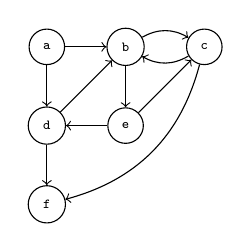
\begin{tikzpicture}[]
\node[draw, circle] (a) at (0, 0) {\tiny \texttt{a}};
\node[draw, circle] (b) at (1, 0) {\tiny \texttt{b}};
\node[draw, circle] (c) at (2, 0) {\tiny \texttt{c}};
\node[draw, circle] (e) at (1, -1) {\tiny \texttt{e}};
\node[draw, circle] (f) at (0, -2) {\tiny \texttt{f}};
\node[draw, circle] (d) at (0, -1) {\tiny \texttt{d}};

\draw[->] (a) -- (b);
\draw[->] (b) edge[bend left] (c);
\draw[->] (b) -- (e);
\draw[->] (c) edge[bend left] (f);
\draw[->] (e) -- (d);


\draw[->] (c) edge[bend left] (b);
\draw[->] (d) edge[] (b);

\draw[->] (a) edge[] (d);
\draw[->] (e) edge[] (c);
\draw[->] (d) edge[] (f);
\end{tikzpicture}

&

\quad

&

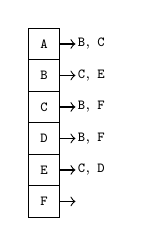
\begin{tikzpicture}[scale = 0.4]
\draw (0, 0) grid (1, 6);
\node at (0.5, 0.5) {\tiny \texttt{F}};
\node at (0.5, 1.5) {\tiny \texttt{E}};
\node at (0.5, 2.5) {\tiny \texttt{D}};
\node at (0.5, 3.5) {\tiny \texttt{C}};
\node at (0.5, 4.5) {\tiny \texttt{B}};
\node at (0.5, 5.5) {\tiny \texttt{A}};

\draw[->] (1, 0.5) -- (1.5, 0.5);
\draw[->] (1, 1.5) -- (1.5, 1.5);
\draw[->] (1, 2.5) -- (1.5, 2.5);
\draw[->] (1, 3.5) -- (1.5, 3.5);
\draw[->] (1, 4.5) -- (1.5, 4.5);
\draw[->] (1, 5.5) -- (1.5, 5.5);


\node at (2, 5.5) {\tiny \texttt{B}, \texttt{C}};
\node at (2, 4.5) {\tiny \texttt{C}, \texttt{E}};
\node at (2, 3.5) {\tiny \texttt{B}, \texttt{F}};
\node at (2, 2.5) {\tiny \texttt{B}, \texttt{F}};
\node at (2, 1.5) {\tiny \texttt{C}, \texttt{D}};
\end{tikzpicture}

\end{tabular}
\end{center}

DFS execution from node \texttt{a}

\begin{center}
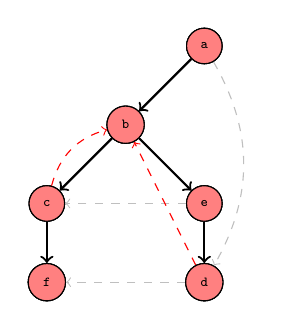
\begin{tikzpicture}[]

\node[draw, circle] (a) at (0, 0) {\tiny \texttt{a}};

\pause

\node[draw, fill = green!50!white, circle] (a) at (0, 0) {\tiny \texttt{a}};

\pause

\node[draw, circle] (b) at (-1, -1) {\tiny \texttt{b}};
\draw[->, thick] (a) -- (b);

\pause

\node[draw, fill = green!50!white, circle] (b) at (-1, -1) {\tiny \texttt{b}};

\pause

\node[draw, circle] (c) at (-2, -2) {\tiny \texttt{c}};
\draw[->, thick] (b) -- (c);

\pause 

\node[draw, fill = green!50!white, circle] (c) at (-2, -2) {\tiny \texttt{c}};

\pause

\draw[->, dashed, red] (c) edge[bend left] (b);

\pause

\node[draw, circle] (f) at (-2, -3) {\tiny \texttt{f}};
\draw[->, thick] (c) -- (f);

\pause

\node[draw, fill = green!50!white, circle] (f) at (-2, -3) {\tiny \texttt{f}};

\pause

\node[draw, fill = red!50!white, circle] (f) at (-2, -3) {\tiny \texttt{f}};

\pause

\node[draw, fill = red!50!white, circle] (c) at (-2, -2) {\tiny \texttt{c}};

\pause

\node[draw, circle] (e) at (0, -2) {\tiny \texttt{e}};
\draw[->, thick] (b) -- (e);

\pause

\node[draw, fill = green!50!white, circle] (e) at (0, -2) {\tiny \texttt{e}};

\pause

\draw[->, dashed, gray!50!white] (e) edge[] (c);

\pause

\node[draw, circle] (d) at (0, -3) {\tiny \texttt{d}};
\draw[->, thick] (e) -- (d);

\pause

\node[draw, fill = green!50!white, circle] (d) at (0, -3) {\tiny \texttt{d}};

\pause

\draw[->, dashed, red] (d) edge[] (b);

\pause 

\draw[->, dashed, gray!50!white] (d) edge[] (f);

\pause

\node[draw, fill = red!50!white, circle] (d) at (0, -3) {\tiny \texttt{d}};

\pause

\node[draw, fill = red!50!white, circle] (e) at (0, -2) {\tiny \texttt{e}};

\pause

\node[draw, fill = red!50!white, circle] (b) at (-1, -1) {\tiny \texttt{b}};

\pause

\draw[->, dashed, gray!50!white] (a) edge[bend left] (d);

\pause


\node[draw, fill = red!50!white, circle] (a) at (0, 0) {\tiny \texttt{a}};



\end{tikzpicture}
\end{center}

\end{frame}
%%%%%%%%%%%%%%%%%%%%%%%%%%%%%%%%%%%%%%%%%%%

\section{Cycle detection}

\begin{frame}

Let's start with \textbf{cycles}.

\vspace{0.5cm}

How can we detect with DFS whether a graph is acyclic or not? \pause

\begin{center}
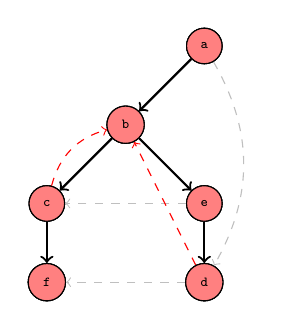
\begin{tikzpicture}[]

\node[draw, circle] (a) at (0, 0) {\tiny \texttt{a}};

\node[draw, fill = green!50!white, circle] (a) at (0, 0) {\tiny \texttt{a}};

\node[draw, circle] (b) at (-1, -1) {\tiny \texttt{b}};
\draw[->, thick] (a) -- (b);

\node[draw, fill = green!50!white, circle] (b) at (-1, -1) {\tiny \texttt{b}};

\node[draw, circle] (c) at (-2, -2) {\tiny \texttt{c}};
\draw[->, thick] (b) -- (c);

\node[draw, fill = green!50!white, circle] (c) at (-2, -2) {\tiny \texttt{c}};

\draw[->, dashed, red] (c) edge[bend left] (b);

\node[draw, circle] (f) at (-2, -3) {\tiny \texttt{f}};
\draw[->, thick] (c) -- (f);

\node[draw, fill = green!50!white, circle] (f) at (-2, -3) {\tiny \texttt{f}};

\node[draw, fill = red!50!white, circle] (f) at (-2, -3) {\tiny \texttt{f}};

\node[draw, fill = red!50!white, circle] (c) at (-2, -2) {\tiny \texttt{c}};

\node[draw, circle] (e) at (0, -2) {\tiny \texttt{e}};
\draw[->, thick] (b) -- (e);

\node[draw, fill = green!50!white, circle] (e) at (0, -2) {\tiny \texttt{e}};

\draw[->, dashed, gray!50!white] (e) edge[] (c);

\node[draw, circle] (d) at (0, -3) {\tiny \texttt{d}};
\draw[->, thick] (e) -- (d);

\node[draw, fill = green!50!white, circle] (d) at (0, -3) {\tiny \texttt{d}};

\draw[->, dashed, red] (d) edge[] (b);

\draw[->, dashed, gray!50!white] (d) edge[] (f);

\node[draw, fill = red!50!white, circle] (d) at (0, -3) {\tiny \texttt{d}};

\node[draw, fill = red!50!white, circle] (e) at (0, -2) {\tiny \texttt{e}};

\node[draw, fill = red!50!white, circle] (b) at (-1, -1) {\tiny \texttt{b}};

\draw[->, dashed, gray!50!white] (a) edge[bend left] (d);


\node[draw, fill = red!50!white, circle] (a) at (0, 0) {\tiny \texttt{a}};



\end{tikzpicture}
\end{center}

The red edges belong to cycles, they are called \textbf{back edges}.

\vspace{0.5cm}

A graph is acyclic if and only if DFS does not yield back edges.

\end{frame}


\begin{frame}

How to distiguish these edges from the others?

\pause 


\begin{center}
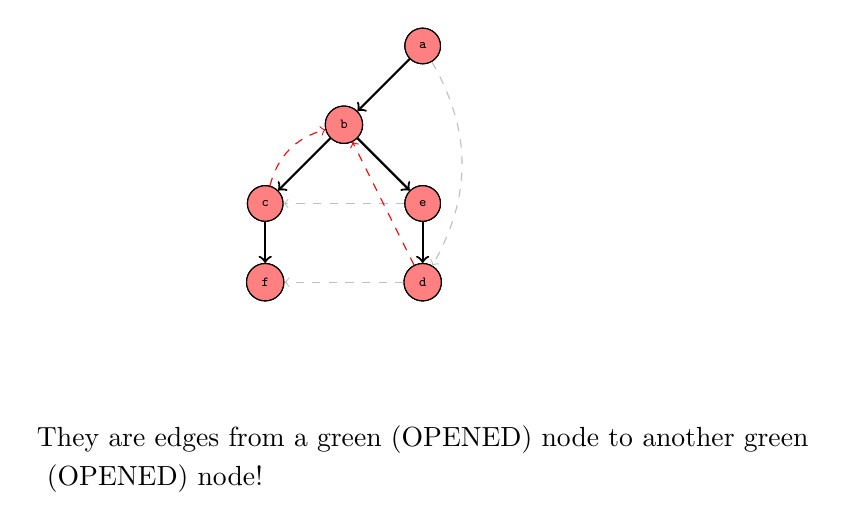
\begin{tikzpicture}[]

\node[draw, circle] (a) at (0, 0) {\tiny \texttt{a}};


\node[draw, fill = green!50!white, circle] (a) at (0, 0) {\tiny \texttt{a}};

\node[draw, circle] (b) at (-1, -1) {\tiny \texttt{b}};
\draw[->, thick] (a) -- (b);

\node[draw, fill = green!50!white, circle] (b) at (-1, -1) {\tiny \texttt{b}};

\node[draw, circle] (c) at (-2, -2) {\tiny \texttt{c}};
\draw[->, thick] (b) -- (c);


\node[draw, fill = green!50!white, circle] (c) at (-2, -2) {\tiny \texttt{c}};

\pause

\draw[->, dashed, red] (c) edge[bend left] (b);

\pause

\node[draw, circle] (f) at (-2, -3) {\tiny \texttt{f}};
\draw[->, thick] (c) -- (f);

\node[draw, fill = green!50!white, circle] (f) at (-2, -3) {\tiny \texttt{f}};

\node[draw, fill = red!50!white, circle] (f) at (-2, -3) {\tiny \texttt{f}};

\node[draw, fill = red!50!white, circle] (c) at (-2, -2) {\tiny \texttt{c}};

\node[draw, circle] (e) at (0, -2) {\tiny \texttt{e}};
\draw[->, thick] (b) -- (e);

\node[draw, fill = green!50!white, circle] (e) at (0, -2) {\tiny \texttt{e}};

\draw[->, dashed, gray!50!white] (e) edge[] (c);

\node[draw, circle] (d) at (0, -3) {\tiny \texttt{d}};
\draw[->, thick] (e) -- (d);

\node[draw, fill = green!50!white, circle] (d) at (0, -3) {\tiny \texttt{d}};

\pause

\draw[->, dashed, red] (d) edge[] (b);

\pause 

\draw[->, dashed, gray!50!white] (d) edge[] (f);

\node[draw, fill = red!50!white, circle] (d) at (0, -3) {\tiny \texttt{d}};

\node[draw, fill = red!50!white, circle] (e) at (0, -2) {\tiny \texttt{e}};

\node[draw, fill = red!50!white, circle] (b) at (-1, -1) {\tiny \texttt{b}};

\draw[->, dashed, gray!50!white] (a) edge[bend left] (d);

\node[draw, fill = red!50!white, circle] (a) at (0, 0) {\tiny \texttt{a}};

\node at (0, -5) {They are edges from a green (OPENED) node to another green};
\node at (-3.4, -5.5) {(OPENED) node!};


\end{tikzpicture}
\end{center}

\end{frame}

\begin{frame}[fragile]

To implement this we simply add a check while listing neighbours.

\vspace{0.5cm}

Checks if node $u$ (which is OPENED) points to another OPENED node.

\vspace{0.5cm}

\begin{lstlisting}
bool hasCycle = false;

void dfs(int u) {
    st[v] = OPENED;
    for (int v : adj[u]) {
        if (st[u] == UNVISITED)
            dfs(v);
        else if (st[u] == OPENED)
            hasCycle = true;
    }
    st[v] = CLOSED;
}
\end{lstlisting}

\end{frame}



\section{Bridges and articulation points}

\begin{frame}

An \textbf{articulation point} in an undirected graph is a node such that its removal disconnects the graph.

\vspace{0.5cm}

A \textbf{bridge} in an undirected graph is an edge such that its removal disconnects the graph.

\vspace{0.5cm}

\begin{center}
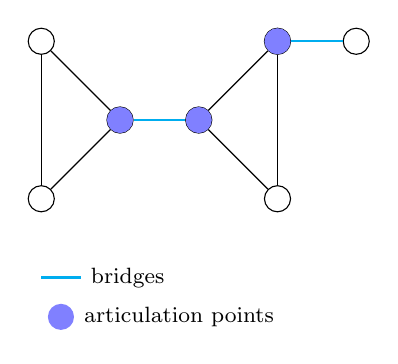
\begin{tikzpicture}

\coordinate (p0) at (0, 1);
\coordinate (p1) at (0, -1);
\coordinate (p2) at (1, 0);
\coordinate (p3) at (2, 0);
\coordinate (p4) at (3, 1);
\coordinate (p5) at (3, -1);
\coordinate (p6) at (4, 1);

\node[draw, circle] (0) at (p0) {};

\node[draw, circle] (1) at (p1) {};
\node[draw, circle] (2) at (p2) {};
\node[draw, circle] (3) at (p3) {};
\node[draw, circle] (4) at (p4) {};
\node[draw, circle] (5) at (p5) {};
\node[draw, circle] (6) at (p6) {};
\draw (0) -- (1);
\draw (0) -- (2);
\draw (2) -- (1);
\draw (2) -- (3);
\draw (3) -- (4);
\draw (3) -- (5);
\draw (4) -- (5);
\draw (4) -- (6);

\pause

\draw[thick, cyan] (2) -- (3);
\draw[thick, cyan] (4) -- (6);

\node[fill = blue!50!white, circle] (2i) at (1, 0) {};
\node[fill = blue!50!white, circle] (3i) at (2, 0) {};
\node[fill = blue!50!white, circle] (4i) at (3, 1) {};

\draw[cyan, thick] (0, -2) -- (0.5, -2) node[black, anchor = west] {\footnotesize bridges};
\node[fill = blue!50!white, circle] at (0.25, -2.5) {};
\node at (1.75, -2.5) {\footnotesize articulation points};

\end{tikzpicture}
\end{center}

\end{frame}

\begin{frame}

How would you compute this?

\pause

\vspace{1cm}

\textbf{Naive algorithm (for bridges):}

\vspace{0.5cm}

For every edge $(x, y)$, remove it and check with \textsf{BFS} or \textsf{DFS} whether $x$ and $y$ remain connected.

\vspace{0.5cm}

Complexity: $O(E \cdot (V + E)) = O(E \cdot V + E^2)$ {\color{red!50!white} TLE} in big graphs.

\vspace{1cm}

We will solve it in \textbf{linear time} with a single DFS.

\end{frame}

\begin{frame}

\textbf{Observation:}

\vspace{0.5cm}

Bridges can never belong to cycles.

\vspace{0.5cm}

Is this true for articulation points? \pause \textbf{NO}.

\vspace{0.5cm}

\begin{center}
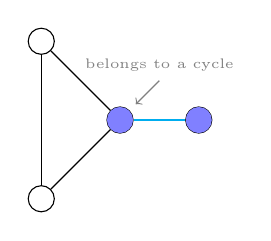
\begin{tikzpicture}
\node[draw, circle] (0) at (0, 1) {};
\node[draw, circle] (1) at (0, -1) {};
\node[draw, circle] (2) at (1, 0) {};
\node[draw, circle] (3) at (2, 0) {};
\draw (0) -- (1);
\draw (0) -- (2);
\draw (2) -- (1);
\draw (2) -- (3);

\draw[thick, cyan] (2) -- (3);

\node[fill = blue!50!white, circle] (2i) at (1, 0) {};
\node[fill = blue!50!white, circle] (3i) at (2, 0) {};

\draw[->, gray] (1.5, 0.5) node[anchor = south, gray] {\tiny belongs to a cycle} -- (1.2, 0.2);

\end{tikzpicture}
\end{center}

\vspace{0.5cm}

So we essentially need to find which edges belong to cycles.

\vspace{0.5cm}

We already say that DFS allows to find cycles.

\end{frame}

%%%%%%%%%%%%%%%%%%%%%%%%%%%%%%%%%%%%%%%%%%%%%%%%%%%%%%%
\begin{frame}

\begin{center}
\begin{tabular}{c c c}

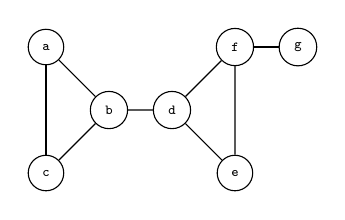
\begin{tikzpicture}[scale = 0.8]
\node[draw, circle] (a) at (0, 0) {\tiny \texttt{a}};
\node[draw, circle] (b) at (1, -1) {\tiny \texttt{b}};
\node[draw, circle] (c) at (0, -2) {\tiny \texttt{c}};
\node[draw, circle] (d) at (2, -1) {\tiny \texttt{d}};
\node[draw, circle] (f) at (3, 0) {\tiny \texttt{f}};
\node[draw, circle] (e) at (3, -2) {\tiny \texttt{e}};
\node[draw, circle] (g) at (4, 0) {\tiny \texttt{g}};

\draw (a) -- (b);
\draw (a) -- (c);
\draw (c) -- (b);
\draw (b) -- (d);
\draw (f) -- (d);
\draw (d) -- (e);
\draw (f) -- (e);
\draw (f) -- (g);

\end{tikzpicture}

&

\quad

&

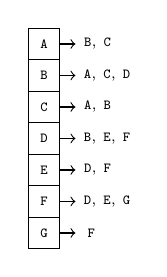
\begin{tikzpicture}[scale = 0.4]
\draw (0, -1) grid (1, 6);
\node at (0.5, -0.5) {\tiny \texttt{G}};
\node at (0.5, 0.5) {\tiny \texttt{F}};
\node at (0.5, 1.5) {\tiny \texttt{E}};
\node at (0.5, 2.5) {\tiny \texttt{D}};
\node at (0.5, 3.5) {\tiny \texttt{C}};
\node at (0.5, 4.5) {\tiny \texttt{B}};
\node at (0.5, 5.5) {\tiny \texttt{A}};

\draw[->] (1, -0.5) -- (1.5, -0.5);
\draw[->] (1, 0.5) -- (1.5, 0.5);
\draw[->] (1, 1.5) -- (1.5, 1.5);
\draw[->] (1, 2.5) -- (1.5, 2.5);
\draw[->] (1, 3.5) -- (1.5, 3.5);
\draw[->] (1, 4.5) -- (1.5, 4.5);
\draw[->] (1, 5.5) -- (1.5, 5.5);


\node at (2.2, 5.5) {\tiny \texttt{B}, \texttt{C}};
\node at (2.5, 4.5) {\tiny \texttt{A}, \texttt{C}, \texttt{D}};
\node at (2.2, 3.5) {\tiny \texttt{A}, \texttt{B}};
\node at (2.5, 2.5) {\tiny \texttt{B}, \texttt{E}, \texttt{F}};
\node at (2.2, 1.5) {\tiny \texttt{D}, \texttt{F}};
\node at (2.5, 0.5) {\tiny \texttt{D}, \texttt{E}, \texttt{G}};
\node at (2, -0.5) {\tiny \texttt{F}};
\end{tikzpicture}

\end{tabular}
\end{center}

DFS execution from node \texttt{a}

\begin{center}
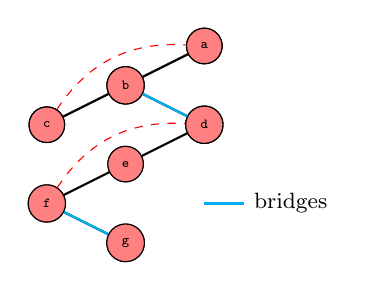
\begin{tikzpicture}[]

\node[draw, circle] (a) at (0, 0) {\tiny \texttt{a}};

\pause

\node[draw, fill = green!50!white, circle] (a) at (0, 0) {\tiny \texttt{a}};

\pause

\node[draw, circle] (b) at (-1, -0.5) {\tiny \texttt{b}};
\draw[thick] (a) -- (b);

\pause

\node[draw, fill = green!50!white, circle] (b) at (-1, -0.5) {\tiny \texttt{b}};

\pause

\node[draw, circle] (c) at (-2, -1) {\tiny \texttt{c}};
\draw[thick] (b) -- (c);

\pause 

\node[draw, fill = green!50!white, circle] (c) at (-2, -1) {\tiny \texttt{c}};

\pause

\draw[dashed, red] (c) edge[bend left] (a);

\pause

\node[draw, fill = red!50!white, circle] (c) at (-2, -1) {\tiny \texttt{c}};

\pause

\node[draw, circle] (d) at (0, -1) {\tiny \texttt{d}};
\draw[thick] (b) -- (d);

\pause

\node[draw, fill = green!50!white, circle] (d) at (0, -1) {\tiny \texttt{d}};

\pause

\node[draw, fill = green!50!white, circle] (e) at (-1, -1.5) {\tiny \texttt{e}};
\draw[thick] (d) -- (e);

\pause

\node[draw, fill = green!50!white, circle] (f) at (-2, -2) {\tiny \texttt{f}};
\draw[thick] (f) -- (e);

\pause

\draw[dashed, red] (f) edge[bend left] (d);

\pause

\node[draw, fill = green!50!white, circle] (g) at (-1, -2.5) {\tiny \texttt{g}};
\draw[thick] (f) -- (g);

\pause

\node[draw, fill = red!50!white, circle] (g) at (-1, -2.5) {\tiny \texttt{g}};

\pause

\node[draw, fill = red!50!white, circle] (f) at (-2, -2) {\tiny \texttt{f}};

\pause

\node[draw, fill = red!50!white, circle] (e) at (-1, -1.5) {\tiny \texttt{e}};

\pause

\node[draw, fill = red!50!white, circle] (d) at (0, -1) {\tiny \texttt{d}};

\pause

\node[draw, fill = red!50!white, circle] (b) at (-1, -0.5) {\tiny \texttt{b}};

\pause

\node[draw, fill = red!50!white, circle] (a) at (0, 0) {\tiny \texttt{a}};

\pause

\draw[thick, cyan] (b) -- (d);
\draw[thick, cyan] (f) -- (g);
\draw[cyan, thick] (0, -2) -- (0.5, -2) node[black, anchor = west] {\footnotesize bridges};



\end{tikzpicture}
\end{center}

\end{frame}
%%%%%%%%%%%%%%%%%%%%%%%%%%%%%%%%%%%%%%%%%%%%%%%%%%%%%%%

\begin{frame}

We observe that an edge $(u, v)$ is a bridge if and only if:

\vspace{0.5cm}

No node in the sub-tree of $v$ has {\color{cyan} a link to $u$ other than $(u,v)$} \textbf{or} {\color{red} a link to one of its ancestors}.

\vspace{0.5cm}

\begin{center}
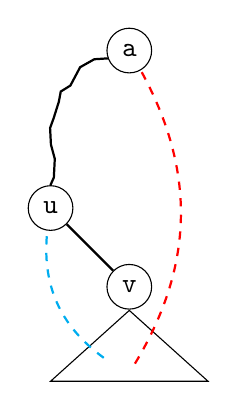
\begin{tikzpicture}[]

\node[draw, circle] (a) at (1, 2) {\texttt{a}};

\node[draw, circle] (u) at (0, 0) {\texttt{u}};
\node[draw, circle] (v) at (1, -1) {\texttt{v}};
\draw[thick] (u) -- (v);

\draw (1, -1.3) -- (0, -2.2) -- (2, -2.2) -- (1, -1.3);
\node at (1, -2.1) (x) {};
\node at (0.8, -2) (y) {};

\draw[thick, dashed, red] (x) edge[bend right] (a);
\draw[thick, dashed, cyan] (y) edge[bend left] (u);

\draw [thick, decorate, decoration={random steps,segment length=5pt,amplitude=2pt}] (a) to[out=200,in=90] (u);

\end{tikzpicture}
\end{center}

What should we add to our DFS to know this information?

\end{frame}


\begin{frame}

We will \textbf{timestamp} the nodes as they are visited: $num$

\vspace{0.5cm}

Keep track of the node with minimum timestamp that we see. We define $low[v]$ as the \textbf{lowest timestamp to which any node in the subtree of $v$ has a direct link}.

\vspace{0.5cm}

$(u, v)$ is a bridge if and only if when we finish $v$, $low[v] > num[u]$

\vspace{0.5cm}

This is so because this means that in the sub-tree of $v$ we did not see any
ancestor of $u$.

\end{frame}

%%%%%%%%%%%%%%%%%%%%%%%%%%%%%%%%%%%%%%%%%%%%%%%%
\begin{frame}

\begin{center}
\begin{tabular}{c c c}

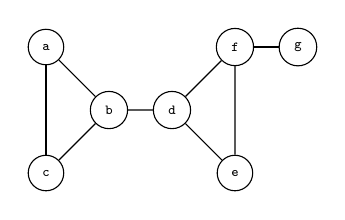
\begin{tikzpicture}[scale = 0.8]
\node[draw, circle] (a) at (0, 0) {\tiny \texttt{a}};
\node[draw, circle] (b) at (1, -1) {\tiny \texttt{b}};
\node[draw, circle] (c) at (0, -2) {\tiny \texttt{c}};
\node[draw, circle] (d) at (2, -1) {\tiny \texttt{d}};
\node[draw, circle] (f) at (3, 0) {\tiny \texttt{f}};
\node[draw, circle] (e) at (3, -2) {\tiny \texttt{e}};
\node[draw, circle] (g) at (4, 0) {\tiny \texttt{g}};

\draw (a) -- (b);
\draw (a) -- (c);
\draw (c) -- (b);
\draw (b) -- (d);
\draw (f) -- (d);
\draw (d) -- (e);
\draw (f) -- (e);
\draw (f) -- (g);

\end{tikzpicture}

&

\quad

&

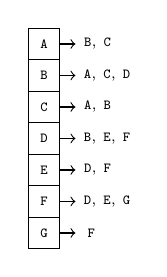
\begin{tikzpicture}[scale = 0.4]
\draw (0, -1) grid (1, 6);
\node at (0.5, -0.5) {\tiny \texttt{G}};
\node at (0.5, 0.5) {\tiny \texttt{F}};
\node at (0.5, 1.5) {\tiny \texttt{E}};
\node at (0.5, 2.5) {\tiny \texttt{D}};
\node at (0.5, 3.5) {\tiny \texttt{C}};
\node at (0.5, 4.5) {\tiny \texttt{B}};
\node at (0.5, 5.5) {\tiny \texttt{A}};

\draw[->] (1, -0.5) -- (1.5, -0.5);
\draw[->] (1, 0.5) -- (1.5, 0.5);
\draw[->] (1, 1.5) -- (1.5, 1.5);
\draw[->] (1, 2.5) -- (1.5, 2.5);
\draw[->] (1, 3.5) -- (1.5, 3.5);
\draw[->] (1, 4.5) -- (1.5, 4.5);
\draw[->] (1, 5.5) -- (1.5, 5.5);


\node at (2.2, 5.5) {\tiny \texttt{B}, \texttt{C}};
\node at (2.5, 4.5) {\tiny \texttt{A}, \texttt{C}, \texttt{D}};
\node at (2.2, 3.5) {\tiny \texttt{A}, \texttt{B}};
\node at (2.5, 2.5) {\tiny \texttt{B}, \texttt{E}, \texttt{F}};
\node at (2.2, 1.5) {\tiny \texttt{D}, \texttt{F}};
\node at (2.5, 0.5) {\tiny \texttt{D}, \texttt{E}, \texttt{G}};
\node at (2, -0.5) {\tiny \texttt{F}};
\end{tikzpicture}

\end{tabular}
\end{center}

DFS execution from node \texttt{a}

\begin{center}
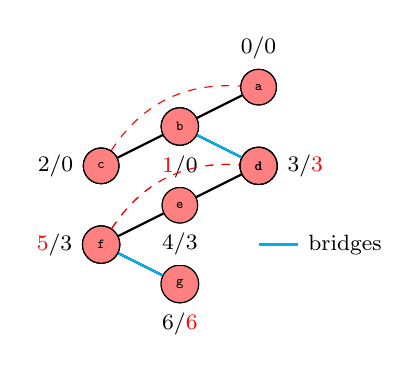
\begin{tikzpicture}[]


\draw[cyan, thick] (0, -2) -- (0.5, -2) node[black, anchor = west] {\footnotesize bridges};
\node[draw, circle] (a) at (0, 0) {\tiny \texttt{a}} node[above = 0.0cm of a, fill = white] {\footnotesize 0/0};

\pause

\node[draw, fill = green!50!white, circle] (a) at (0, 0) {\tiny \texttt{a}} node[above = 0.0cm of a, fill = white] {\footnotesize 0/0};

\pause

\node[draw, circle] (b) at (-1, -0.5) {\tiny \texttt{b}};
\draw[thick] (a) -- (b);


\pause

\node[draw, fill = green!50!white, circle] (b) at (-1, -0.5) {\tiny \texttt{b}} node[below = -0.0cm of b, fill = white] {\footnotesize 1/1};

\pause

\node[draw, circle] (c) at (-2, -1) {\tiny \texttt{c}} node[left = 0.0cm of c, fill = white] {\footnotesize 2/2};
\draw[thick] (b) -- (c);

\pause 

\node[draw, fill = green!50!white, circle] (c) at (-2, -1) {\tiny \texttt{c}} node[left = 0.0cm of c, fill = white] {\footnotesize 2/2};

\pause

\draw[dashed, red] (c) edge[bend left] (a);
\node[draw, fill = green!50!white, circle] (c) at (-2, -1) {\tiny \texttt{c}} node[left = 0.0cm of c, fill = white] {\footnotesize 2/0};

\pause

\node[draw, fill = red!50!white, circle] (c) at (-2, -1) {\tiny \texttt{c}} node[left = 0.0cm of c, fill = white] {\footnotesize 2/0};
\node[draw, fill = green!50!white, circle] (b) at (-1, -0.5) {\tiny \texttt{b}} node[below = 0.0cm of b, fill = white] {\footnotesize 1/0};

\pause

\node[draw, circle] (d) at (0, -1) {\tiny \texttt{d}} node[right = 0.0cm of d, fill = white] {\footnotesize 3/3};
\draw[thick] (b) -- (d);

\pause

\node[draw, fill = green!50!white, circle] (d) at (0, -1) {\tiny \texttt{d}} node[right = 0.0cm of d, fill = white] {\footnotesize 3/3};

\pause

\node[draw, fill = green!50!white, circle] (e) at (-1, -1.5) {\tiny \texttt{e}} node[below = 0.0cm of e, fill = white] {\footnotesize 4/4};
\draw[thick] (d) -- (e);

\pause

\node[draw, fill = green!50!white, circle] (f) at (-2, -2) {\tiny \texttt{f}} node[left = 0.0cm of f, fill = white] {\footnotesize 5/5};
\draw[thick] (f) -- (e);

\pause

\node[draw, fill = green!50!white, circle] (f) at (-2, -2) {\tiny \texttt{f}} node[left = 0.0cm of f, fill = white] {\footnotesize 5/3};
\draw[dashed, red] (f) edge[bend left] (d);

\pause

\node[draw, fill = green!50!white, circle] (g) at (-1, -2.5) {\tiny \texttt{g}} node[below = 0.0cm of g, fill = white] {\footnotesize 6/6};
\draw[thick] (f) -- (g);

\pause

\node[draw, fill = red!50!white, circle] (g) at (-1, -2.5) {\tiny \texttt{g}} node[below = 0.0cm of g, fill = white] {\footnotesize 6/{\color{red}6}};
\node[draw, fill = green!50!white, circle] (f) at (-2, -2) {\tiny \texttt{f}} node[left = 0.0cm of f, fill = white] {\footnotesize {\color{red}5}/3};
\draw[thick, cyan] (f) -- (g);

\pause

\node[draw, fill = red!50!white, circle] (f) at (-2, -2) {\tiny \texttt{f}};

\pause

\node[draw, fill = red!50!white, circle] (e) at (-1, -1.5) {\tiny \texttt{e}} node[below = 0.0cm of e, fill = white] {\footnotesize 4/3};

\pause

\node[draw, fill = red!50!white, circle] (d) at (0, -1) {\tiny \texttt{d}};

\pause

\node[draw, fill = red!50!white, circle] (b) at (-1, -0.5) {\tiny \texttt{b}}  node[below = -0.0cm of b, fill = white] {\footnotesize {\color{red}1}/0};
\node[draw, circle] (d) at (0, -1) {\tiny \texttt{d}} node[right = 0.0cm of d, fill = white] {\footnotesize 3/{\color{red}3}};
\draw[dashed, red] (f) edge[bend left] (d);

\draw[thick, cyan] (b) -- (d);
\pause

\node[draw, fill = red!50!white, circle] (a) at (0, 0) {\tiny \texttt{a}};

\end{tikzpicture}
\end{center}
\end{frame}

%%%%%%%%%%%%%%%%%%%%%%%%%%%%%%%%%%%%%%%%%%%%%%%%

\begin{frame}

So what about \textbf{articulation points}? \pause

\vspace{0.5cm}

We observe that a node $u$ is an articulation point if and only if:

\vspace{0.5cm}

No node in the sub-tree of $v$ has a link to {\color{red} a (strict) ancestor of $u$}.

\vspace{0.5cm}

\begin{center}
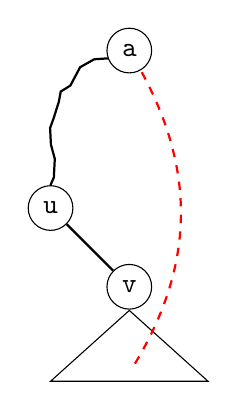
\begin{tikzpicture}[]

\node[draw, circle] (a) at (1, 2) {\texttt{a}};

\node[draw, circle] (u) at (0, 0) {\texttt{u}};
\node[draw, circle] (v) at (1, -1) {\texttt{v}};
\draw[thick] (u) -- (v);

\draw (1, -1.3) -- (0, -2.2) -- (2, -2.2) -- (1, -1.3);
\node at (1, -2.1) (x) {};
\node at (0.8, -2) (y) {};

\draw[thick, dashed, red] (x) edge[bend right] (a);
%\draw[thick, dashed, cyan] (y) edge[bend left] (u);

%\draw[dashed] (a) edge[bend right] (u);

\draw [thick, decorate, decoration={random steps,segment length=5pt,amplitude=2pt}] (a) to[out=200,in=90] (u);

\end{tikzpicture}
\end{center}

Note that a link to $u$ does not help here.
 
\end{frame}

\begin{frame}

What does this mean in terms of $num$ and $low$? \pause

\vspace{0.5cm}

A non-root node $u$ is an articulation point if and only if when we finish $v$, $low[v] \geq num[u]$.\footnote{Note that this might be detected several times with different children $v$, so don't output it directly!}

\begin{center}
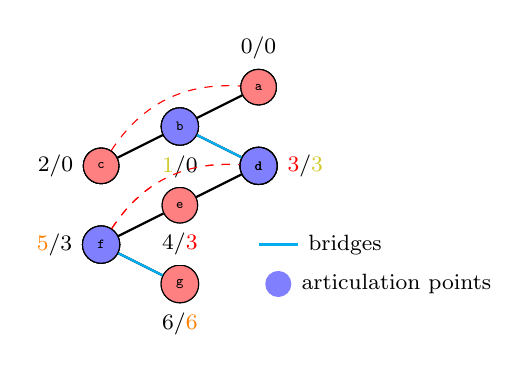
\begin{tikzpicture}[]

\node[fill = blue!50!white, circle] at (0.25, -2.5) {};
\node at (1.75, -2.5) {\footnotesize articulation points};

\draw[cyan, thick] (0, -2) -- (0.5, -2) node[black, anchor = west] {\footnotesize bridges};
\node[draw, circle] (a) at (0, 0) {\tiny \texttt{a}} node[above = 0.0cm of a, fill = white] {\footnotesize 0/0};

\node[draw, fill = green!50!white, circle] (a) at (0, 0) {\tiny \texttt{a}} node[above = 0.0cm of a, fill = white] {\footnotesize 0/0};

\node[draw, circle] (b) at (-1, -0.5) {\tiny \texttt{b}};
\draw[thick] (a) -- (b);

\node[draw, fill = green!50!white, circle] (b) at (-1, -0.5) {\tiny \texttt{b}} node[below = -0.0cm of b, fill = white] {\footnotesize 1/1};

\node[draw, circle] (c) at (-2, -1) {\tiny \texttt{c}} node[left = 0.0cm of c, fill = white] {\footnotesize 2/2};
\draw[thick] (b) -- (c);

\node[draw, fill = green!50!white, circle] (c) at (-2, -1) {\tiny \texttt{c}} node[left = 0.0cm of c, fill = white] {\footnotesize 2/2};

\draw[dashed, red] (c) edge[bend left] (a);
\node[draw, fill = green!50!white, circle] (c) at (-2, -1) {\tiny \texttt{c}} node[left = 0.0cm of c, fill = white] {\footnotesize 2/0};

\node[draw, fill = red!50!white, circle] (c) at (-2, -1) {\tiny \texttt{c}} node[left = 0.0cm of c, fill = white] {\footnotesize 2/0};
\node[draw, fill = green!50!white, circle] (b) at (-1, -0.5) {\tiny \texttt{b}} node[below = 0.0cm of b, fill = white] {\footnotesize 1/0};

\node[draw, circle] (d) at (0, -1) {\tiny \texttt{d}} node[right = 0.0cm of d, fill = white] {\footnotesize 3/3};
\draw[thick] (b) -- (d);

\node[draw, fill = green!50!white, circle] (d) at (0, -1) {\tiny \texttt{d}} node[right = 0.0cm of d, fill = white] {\footnotesize 3/3};

\node[draw, fill = green!50!white, circle] (e) at (-1, -1.5) {\tiny \texttt{e}} node[below = 0.0cm of e, fill = white] {\footnotesize 4/4};
\draw[thick] (d) -- (e);

\node[draw, fill = green!50!white, circle] (f) at (-2, -2) {\tiny \texttt{f}} node[left = 0.0cm of f, fill = white] {\footnotesize 5/5};
\draw[thick] (f) -- (e);

\node[draw, fill = green!50!white, circle] (f) at (-2, -2) {\tiny \texttt{f}} node[left = 0.0cm of f, fill = white] {\footnotesize 5/3};
\draw[dashed, red] (f) edge[bend left] (d);

\node[draw, fill = green!50!white, circle] (g) at (-1, -2.5) {\tiny \texttt{g}} node[below = 0.0cm of g, fill = white] {\footnotesize 6/6};
\draw[thick] (f) -- (g);

\node[draw, fill = red!50!white, circle] (g) at (-1, -2.5) {\tiny \texttt{g}} node[below = 0.0cm of g, fill = white] {\footnotesize 6/{\color{orange}6}};
\node[draw, fill = green!50!white, circle] (f) at (-2, -2) {\tiny \texttt{f}} node[left = 0.0cm of f, fill = white] {\footnotesize {\color{orange}5}/3};
\draw[thick, cyan] (f) -- (g);

\node[draw, fill = blue!50!white, circle] (f) at (-2, -2) {\tiny \texttt{f}};

\node[draw, fill = red!50!white, circle] (e) at (-1, -1.5) {\tiny \texttt{e}} node[below = 0.0cm of e, fill = white] {\footnotesize 4/{\color{red}3}};

\node[draw, fill = blue!50!white, circle] (d) at (0, -1) {\tiny \texttt{d}};

\node[draw, fill = blue!50!white, circle] (b) at (-1, -0.5) {\tiny \texttt{b}}  node[below = -0.0cm of b, fill = white] {\footnotesize {\color{yellow!80!black}1}/0};
\node[draw, circle] (d) at (0, -1) {\tiny \texttt{d}} node[right = 0.0cm of d, fill = white] {\footnotesize {\color{red}3}/{\color{yellow!80!black}3}};
\draw[dashed, red] (f) edge[bend left] (d);

\draw[thick, cyan] (b) -- (d);

\node[draw, fill = red!50!white, circle] (a) at (0, 0) {\tiny \texttt{a}};



\end{tikzpicture}
\end{center}


\end{frame}

\begin{frame}

What about the root? \pause 

\vspace{0.5cm}

Root is articulation if and only if it has more than one child.

\vspace{0.5cm}

\begin{center}
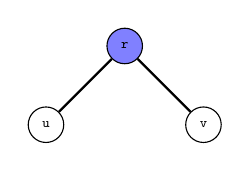
\begin{tikzpicture}
\node[draw, circle, fill = blue!50!white] (r) at (0, 0) {\tiny \texttt{r}};
\node[draw, circle] (u) at (-1, -1) {\tiny \texttt{u}};
\node[draw, circle] (v) at (1, -1) {\tiny \texttt{v}};

\draw[thick] (r) -- (u);
\draw[thick] (r) -- (v);

\end{tikzpicture}
\end{center}

\vspace{0.5cm}

Removing node $r$ disconnects the graph.

\vspace{0.5cm}

If there was another path from $u$ to $v$, $v$ would not be a child of $r$.

\end{frame}


\begin{frame}[fragile]

\begin{lstlisting}
int num[N], low[N], root, rootChildren, cnt = 0;

void dfs(int u, int parent) {
    num[u] = low[u] = cnt++;
    vis[u] = true;
    for (int v : adj[u]) {
        if (!vis[v]) {
            dfs(v, u);
            if (u == root) rootChildren++;
            if (low[v] >= num[u] && u != root)
                // u is an articulation point
            if (low[v] > num[u])
                // (u,v) is a bridge
            low[u] = min(low[u], low[v]);
        } else if (v != parent)
            low[u] = min(low[u], num[v]);
    }
}

// loop in main():
if (!vis[u]) {
    root = u, rootChildren = 0;
    dfs(u, -1);
    if(rootChildren > 1)
        // u is an articulation point
}
\end{lstlisting}

\end{frame}

\end{document}
